% This is samplepaper.tex, a sample chapter demonstrating the
% LLNCS macro package for Springer Computer Science proceedings;
% Version 2.20 of 2017/10/04
%
\documentclass[runningheads]{llncs}
%
\usepackage{amsmath}
\usepackage{amssymb}
\usepackage{booktabs} % For pretty tables
\usepackage{caption} % For caption spacing
\usepackage{subcaption}
\usepackage{graphicx}
\usepackage{pgfplots}
\usepackage[all]{nowidow}
\usepackage[utf8]{inputenc}
\usepackage{tikz}
\usetikzlibrary{er,positioning,bayesnet}
\usepackage{multicol}
\usepackage{algpseudocode,algorithm,algorithmicx}
\usepackage{hyperref}
\usepackage[inline]{enumitem} % Horizontal lists
\newcommand{\indentitem}{\setlength\itemindent{20pt}}

\graphicspath{{latex/}}
\newcommand{\card}[1]{\left\vert{#1}\right\vert}
\newcommand*\Let[2]{\State #1 $\gets$ #2}
\newcommand\qfrac[3][1pt]{\frac{%
		\ThisStyle{\addstackgap[#1]{\SavedStyle#2}}}{%
		\ThisStyle{\addstackgap[#1]{\SavedStyle#3}}%
}}


\newcommand{\F}{\ensuremath{\mathbb{F}}}
\newcommand{\B}{\ensuremath{\mathbb{B}}}
\newcommand{\LL}{\ensuremath{\mathbb{L}}}
\newcommand{\Me}{\ensuremath{\mathbb{M}_e^{\text{eff}}}}
\newcommand{\D}{\ensuremath{\text{D}}}
\renewcommand{\d}{\ensuremath{\text{d}}}
\pgfplotsset{compat=1.14}

\renewcommand{\topfraction}{0.85}
\renewcommand{\bottomfraction}{0.85}
\renewcommand{\textfraction}{0.15}
\renewcommand{\floatpagefraction}{0.8}
\renewcommand{\textfraction}{0.1}
\setlength{\floatsep}{3pt plus 1pt minus 1pt}
\setlength{\textfloatsep}{3pt plus 1pt minus 1pt}
\setlength{\intextsep}{3pt plus 1pt minus 1pt}
\setlength{\abovecaptionskip}{2pt plus 1pt minus 1pt}


\begin{document}
%
\title{A thermodynamically consistent poro-visco-elastic model of Extracellular Matrix}
%
\titlerunning{Mechanical Properties of ECM}
% If the paper title is too long for the running head, you can set
% an abbreviated paper title here
%
\author{Giulia Laura Celora}
%
%\authorrunning{F. Author et al.}
% First names are abbreviated in the running head.
% If there are more than two authors, 'et al.' is used.
%
\institute{Mathematical Institute, University of Oxford}
%
\maketitle              % typeset the header of the contribution
%
\begin{abstract}

\end{abstract}
%
%
%
\section{Introduction}

There are several studies supporting the central role of mechanical stimuli in tissue morphogenesis and homeostasis \cite{ex1,ex2}. In tissues, cells are mainly surrounded by extracellular matrix (ECM), a soft porous media made up of  networks of polymer chains and proteins. \textit{In vitro} studies have shown that ECM rigidity and shear stresses can alone promote malignant phenotypes in a population of initially normal cells, impact on cell proliferation and differentiation \cite{ex3}. Further experiments on solid tumour development have proven that this is often associated to a stiffening of the tissue compared to the surrounding healthy one \cite{ex4}, which results in the exposure of cells to higher compressive stresses as well as favouring the collapse of blood vessels and impeding the diffusion of substances in the extra-cellular environment ultimately decreasing the efficacy of numerous therapies \cite{ecm2}. Based on such evidence, it is now widely accepted that, unlike originally thought, biological process are not simply regulated by biochemical signals but by the complex interplay of mechanical and chemical stimuli.
 
Given the different physical nature and scale of phenomena involved, coupling micro-environment and cell behaviours is a problem of high complexity. This requires understanding processes occurring at different temporal and spatial scales and how they interplay to determine the macroscopic behaviour of a tissue, whether healthy or damaged. If we can learn to tune its properties, as cells already do, this could led to the development of novel therapies and completely change our approach to  drug design. In order for this to be possible, alongside experiments, it is necessary to develop a theoretical framework able to capture both the biology and physics involved and which is consistent with the known universal laws of Nature \cite{NET}. 

With the development of new experimental techniques such as Atomic Force Microscopy (AFM), the local mechanical properties of a material can be measured with atomic precision \cite{viscoporo}. When tested at this scale, soft tissues and the ECM in particular have been found to be visco-elastic \cite{ex5}. Purely elastic solids only store energy when deformed, viscoelastic material instead exhibit a time-dependent response as part of the energy is dissipated in the deformation process. While a large amount of literature focuses on the elastic properties of ECM, it remains unclear the role of viscosity in determining cell behaviour. However, the recent efforts to develop synthetic ECM, i.e. hydrogels, with tunable viscoelasticity, have now opened new research opportunities \cite{viscocell}. 

Despite the progress in experimental techniques, theoretical studies of viscoelastic soft materials remain limited. While experiments rapidly progress, most of the literature on mathematical modelling for soft matter has completely neglected viscous dissipation \cite{Article1}. Whether this assumption might be valid for certain applications, the empirical studies previously mentioned highlight the need of including this component in the study of living tissues. Our works aims to develop a continuum mathematical model of the extracellular matrix which is consistent with the laws of thermodynamics, which accounts for its poro-visco-elastic properties and the coupling of mechanical, transport and electrical phenomena. At our present knowledge, there is no previous work in the literature capturing all these aspects. In \cite{ecm1,ecm2} Xue et al.~ develop a nonlinear poroelastic theory for ECM, which couples all three physical phenomena but does not include viscous dissipation. In \cite{Jeru}, the authors couple mechano-electrophysiological effects including the viscous dissipation but neglect transport; Caccavo et al.~ \cite{Article1} propose a poro-viscoelastic model for neutral hydrogel, thus excluding electrical effects.  Following these previous work, we will derive our model in the framework of linear non-equilibrium thermodynamics \cite{NET}, multi-phase modelling and Biot's poroelastic theory of continuum \cite{Biot}. 

Despite the large number of studies that have characterised the poro-elastic and visco-elastic properties of ECM independently, little is known about their combined effect. In the literature, two main constitutive models have been presented, but never rigorously compared.  Instead of arbitrarily choosing one of the two, we here rely on both approaches, with the aim of identifying their differences and investigating experimental result which would allow us to experimentally test which one best describes the behaviour of soft tissues. From this point of view, our results are more widely applicable to the study of polyelectrolyte gels, which are largely applied as biomedical devices and as a synthetic equivalent of ECM.

Our work is organized as follows: in Section \ref{secNET} we start with a brief overview of Classical Irreversible Thermodynamics. After presenting the composition of the ECM, Section \ref{modeldev} will be focusing on the derivation of the governing equation for the deformation and swelling of ECM. [... FOLLOWING SECTIONS TO UPDATE AS I WRITE.]

\section{Non Equilibrium Thermodynamics.}
\label{secNET}
While equilibrium thermodynamics can describe ideal processes, it does not apply to real processes which are irreversible. In this cases, the change in the entropy of a system $\d S$ results from both the reversible exchange of energy and matter with the external environment $\d_eS$ and the internal dissipation of energy during the process $\d_iS$ \cite{NET}:
\begin{equation}
\d S = \d_eS + \d_iS, 
\end{equation}
According to the second law of thermodynamics, which applies universally to any system or any of its sub-part $\d S_i\ge 0$. It is important to notice that the second law allows transformations in which total change in entropy $d S$ of the system is negative. This occurs whenever $-\d_e S>\d_i S$ and it can lead to the spontaneous formation of complex and ordered structures such as living organisms. From this point of view, life has emerged as an efficient mechanism able to increase sufficiently the entropy of its environment \cite{JeremyEngland}.  

In this study, we will focus on isothermal processes, i.e. $T=const$. Under this assumption, as derived by Gurtin in \cite{GURTIN}, the second law of thermodynamics is equivalent to the following \textit{energy imbalance inequality}:
\begin{equation}
\frac{\d}{\d t} \left\{\int_R \psi \right\}\leq W(R) + M(R) \label{energyin}
\end{equation}
where $R$ is a arbitrary control volume of the system, $\psi$ is the Helmholtz free energy, $W(R)$ is the rate at which the environment does work on $R$ and $M(R)$ is the inflow of mass due to transport. It is important to note that, as long as the quantities involved are well defined, the energy inequality~(\ref{energyin}) holds for any isothermal process independently of the specific physical system considered. This imposes a constraint on the form of the function $\psi$ and how this depends on the other thermodynamic variables, such as temperature or pressure, which are used to describe the system. 

Non-equilibrium thermodynamics mainly focuses on defining the form of $\d_i S$, which, unlike the reversible entropy production $\d_e S$, is not a state variable but depends on the specific transformation applied to the system. 
Different theories have been proposed, \cite{NET}, each with its assumptions and specific domain of applicability. In our study we will focus on \textquotedblleft Classical Irreversible Thermodynamics'' (CIT) which was pioneered by Onsager \cite{onsager} and Prigogine \cite{prigogine} in the first half of the 20th century. One the most important assumptions of this theory is the \textit{Local Equilibrium Hypothesis}, which guarantees thermodynamic variables, including entropy, are locally well-defined, \cite{NET}. 
Consequently, we can introduce the entropy density $s=s(\mathbf{x},t)$ such that:
\begin{equation}
S = \int_{R} s \,\d V, \qquad \d s = \d_e s + \d_is, \qquad \d_is > 0, 
\end{equation}
and the local entropy production:
\begin{equation}
\sigma \equiv \frac{\d_i s}{\d t} \geq 0.
\end{equation}

Another central aspect of the theory is the introduction of \textit{thermodynamic forces} \footnote{Not to be intended in the mechanical sense} $F_m$ (causes) and \textit{thermodynamic fluxes} $J_m$ (effects) to describe the time evolution of the system during an irreversible transformation. These are related to $\sigma$ as follows:
\begin{equation}
\sigma = \sum_m F_m J_m.
\label{2law}
\end{equation}

While the local equilibrium hypothesis is at the basis of most theories of non-equilibrium thermodynamics, the following two hypotheses uniquely identify CIT:
\begin{itemize}
	\item[1.] \textit{Linear Relation between forces $F$ and fluxes $J$}:
	\begin{equation}
	J_m = \sum_k L_{mk} F_k,\label{lin}
	\end{equation}
	where the constant $L_{mk}$ are referred to as \textbf{phenomenological coefficients};
	\item[2.] \textit{Microscopic Reversibility}: time reversibility of processes at the micro-scale. 
\end{itemize}

Starting from these two principles, in its seminal paper \cite{onsager} Onsager derives the well-known \textit{Onsager Reciprocal Relation}:
\begin{equation}
L_{mk}=L_{km}.
\end{equation}

If we now consider an isothermal transformation in the framework of CIT, alongside with the energy imbalance inequality, we have that the following must hold:

\begin{equation}
W(R)+M(R)-\frac{\d}{\d t} \left\{\int_R \psi \right\} = T \int_R \sigma \,\d V\, ,
\label{eqCIT}
\end{equation}

In the past few decades, CIT has been applied successfully to the modelling of several physical phenomena of interest for engineers, physicists and applied mathematicians. However, its validity is limited to phenomena near-equilibrium, for which a linear approximation of the flux-force relation holds. The growing interest in more complex far-from-equilibrium phenomena has pushed toward the development of a more general framework for the study of a non-equilibrium phenomena. Since this goes beyond the purpose of our study, we will not discuss it further. We just want to mention the law of steepest entropy ascent, which, according to Beretta \cite{SEA2}, seems to emerge as the fourth fundamental law of nature. In the linear regime, this principle can be used to prove Onsager's reciprocal relation \cite{SEA1}, with no reference to the microscopic reversibility hypothesis, whose validity remains instead controversial \cite{CIT}.

\section{Composition of Extracellular Matrix.}
\label{ECMcomp}
Despite the tissue-specific nature of Extracellular Matrix (ECM), as shown in Figure \ref{ECMfig} (a), this is usually composed of a network of collagen fibrils entangled with proteoglycans (PGAs) which are covalently bonded to charged chains of glycosaminoglycans (GAGs).  While collagen is mainly responsible for the mechanical behaviour of the tissue, GAGs can imbibe water, giving the extracellular matrix the ability to swell while maintaining its structural integrity. From this point of view, the ECM behaves as a polyelectrolyte gel \cite{ecm1,ecm2}. As schematically illustrated in Figure \ref{ECMfig}(b), polyelectrolyte gels are 3D networks of cross-linked polymer chains that contain ionizable functional groups. When in solution the gel swells, while the functional groups dissociate into fixed charges and mobile ions in the solution. Besides being largely present in the natural world, synthetic polyelectrolytes are currently employed for a wide range of applications, such as drug delivery, biomedical devices, scaffolds for tissue engineering and soft robotics \cite{hydroex3,hydroex2,hydroex1,hydroex4}. Given their wide industrial application, there has been a growing effort in understanding their behaviour and translating it into mathematical models. In particular, research has been focusing on the phenomena of swelling, i.e. large deformation due to absorption of water, and the diffusion transport and release of solution  \cite{DROZDOV+,DROZDOVph,Reviewpolyel,swell2}. However, only a small fraction of the study published accounts for the visco-elastic properties of the polymer network.
\vspace{4mm}
\begin{figure}[h]
	\begin{subfigure}{0.49\textwidth}
	\centering
	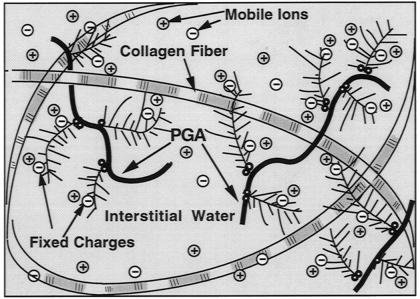
\includegraphics[scale=0.3]{images/ECM}
	\caption{}
	\end{subfigure}
	\begin{subfigure}{0.49\textwidth}
	\centering
	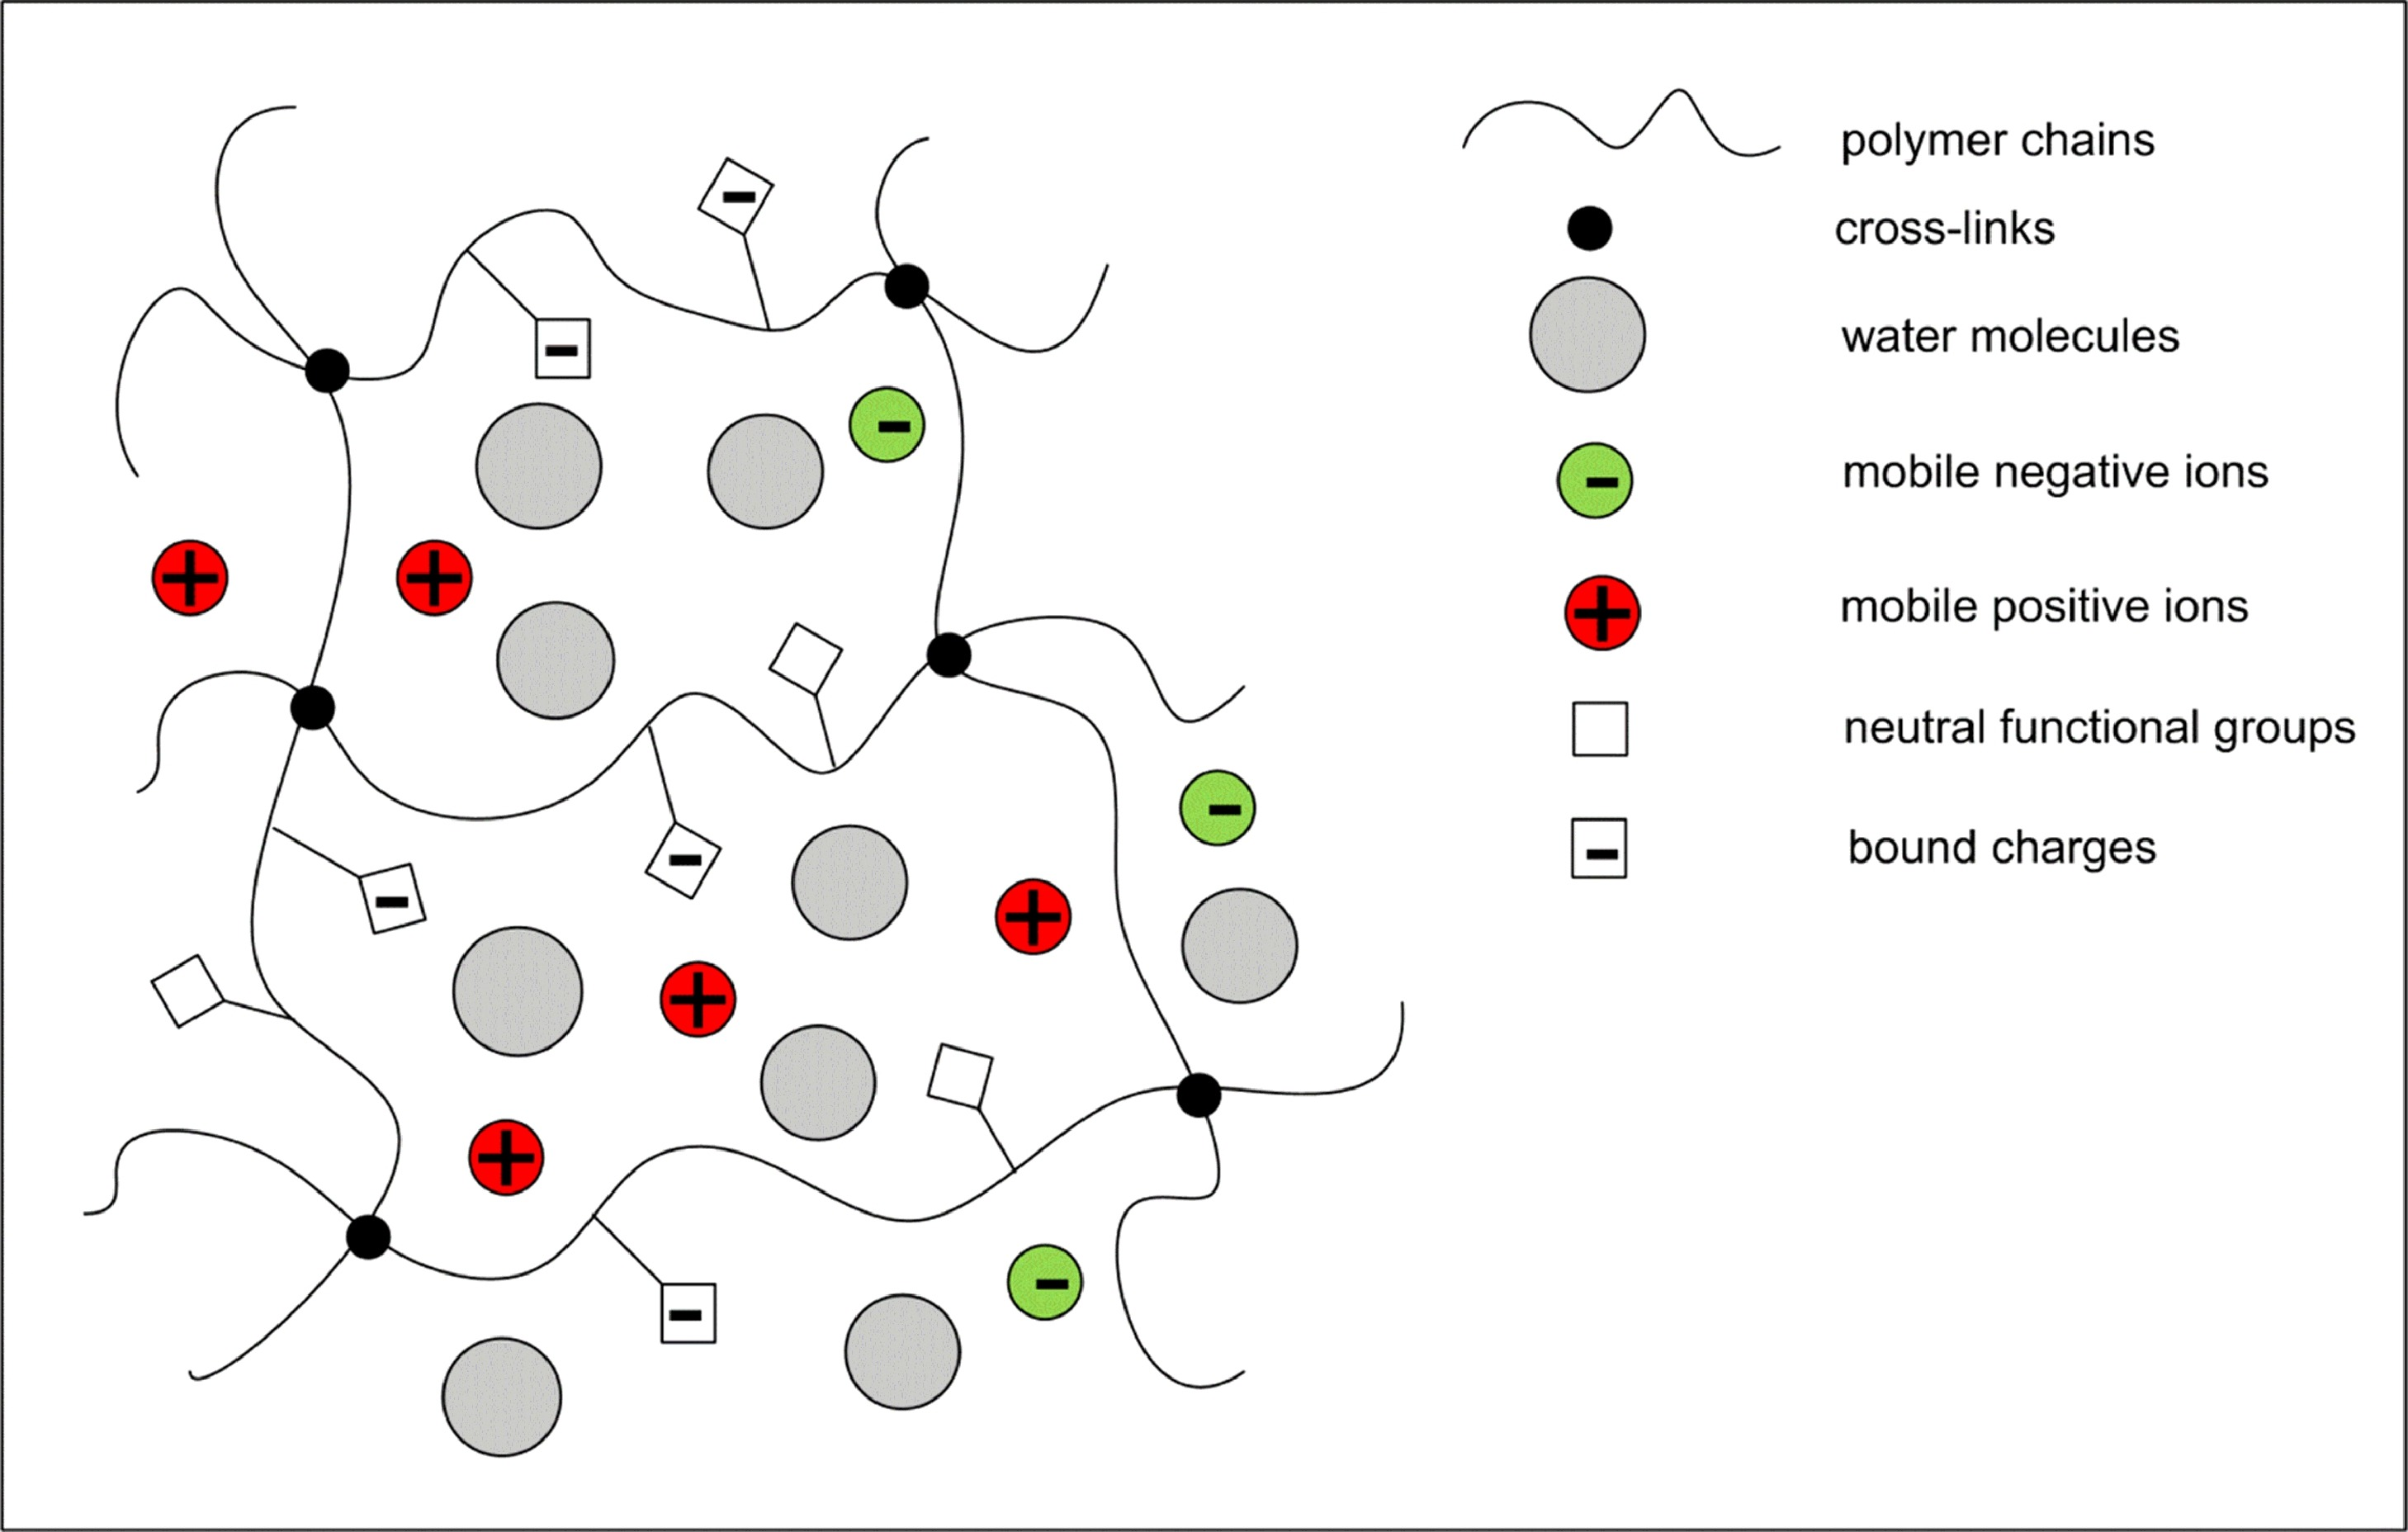
\includegraphics[scale=0.32]{images/ecmscheme.jpg}
	\caption{}
\end{subfigure}
\caption{Analogy between ECM in soft tissue and polyelectrolytes hydrogels: (a) schematic diagram of the structure of the charged hydrated articular cartilage, reproduced from \cite{pictureECM}; (b) an anionic polyelectrolyte gel modelled as a three-phase continuum, reproduced from \cite{DROZDOVph}.}
\label{ECMfig}
\end{figure}
\vspace{2mm}
As shown in Figure \ref{ECMfig}, the extracellular matrix falls into the definition of polyelectrolytes so that the knowledge acquired in the study of these materials can be transferred to soft tissues. For the purpose of this study, we will not explicitly distinguish between collagen, PGAs and GAGs. At the tissue level, this can be grouped into a single solid phase (the polymer networks), whose mechanical properties are treated as the average over the different components contribution. As common in multiphase models of tissue, we will assume that the matrix is isotropic and GAGs are evenly distributed on the network. While this is not a good approximation for tissue like cartilage, which are highly anisotropic, it does apply to the extracellular matrix found in other soft tissue like liver, brain and tumours. It is also important to point out that ECM has additional properties such as thermo-sensitivity and pH-sensitivity. However, both in living organisms and in experimental set-up temperature and pH are maintained fairly constant.

\section{Model Development}
\label{modeldev}
\subsection{Conservation Law.}
\label{conslaw}
As mentioned in the previous section, we here consider the ECM as a three-phase medium composed of a solid polymer network with fixed charges, a solvent (i.e. water molecules, interstitial fluid) and solutes (freely moving charges). 

We assume that the deformation of the ECM corresponds to the one of the solid network. As the tissue deform, the material element originally located at $\mathbf{X}$ in the initial configuration $\mathcal{B}_0$ is displaced to the point $\mathbf{x}$ in the current configuration $\mathcal{B}$. Such transformation is described by the deformation gradient tensor $\F= \partial \mathbf{x}/\partial \mathbf{X}$; the information about the change in ECM's volume due is encoded by $J= \det \F$. Since we assume the solid phase to be incompressible, any change in the volume can only be related to the migration of solvent and solutes molecules, whose nominal concentrations will be denoted by $C_s$ and $C_i$ respectively, $i=1,\ldots,N$ with $N$ being the number of free ion species. This lead to the molecular incompressibility condition:

\begin{equation}
 J= 1 + v_s C_s +\sum\limits_{i=1}^{N} v_i C_i
 \label{comp}
\end{equation}
where $v_m$ are the characteristic molecular volume of each species in the solution. When considering the interstitial fluid, the contribution of ions to the volume can be neglected \cite{ecm1,ecm2} so that Equation~(\ref{comp}) reduces to:

\begin{equation}
J=1+v_s C_s.
\label{inc}
\end{equation} 

Consequently, the volume fractions of fluid $\phi_f$ and solid $\phi_n$ phases in the gel are defined as:
\begin{equation}
\phi_f = \frac{v_sC_s}{1+v_sC_s}, \qquad \phi_n = \frac{1}{1+v_sC_s}.
\end{equation}
where again we are neglecting the contribution of ions to the total volume.
While $C_m$ denote the number of each molecule per unit volume in the initial configuration for the $m$-th species in the solution, the actual concentration in the current state is denoted by $c_m=C_m/J$. Throughout the derivation of the model, we will be using the index $i=1,\ldots,N$ to denote the ionic species only, while $m\in\left\{s,1,\ldots,N\right\}$ to refer to all mobile species, i.e. both the solvent and solutes.

Mass conservation must apply to all mobile species and in the initial configuration this reads:
\begin{equation}
\dot{C}_m + \nabla_0 \cdot \mathbf{J}_m = 0, \label{consmass}
\end{equation}
where $\mathbf{J}_m$ is the nominal flux per unit area in the dry state and $\nabla_0$ denote the gradient in the Lagrangian coordinates $\mathbf{X}$. Their counterparts in the actual configuration are denoted by $\mathbf{j}_m$ and $\nabla$ and are defined according to the following rules:
\begin{equation}
\mathbf{J}_m = J \F^{-1} \mathbf{j}_m, \qquad \nabla_0 (\cdot) = \F^{T} \nabla(\cdot).
\end{equation}

When considering tissues or hydrogels, inertial and gravitational effect are commonly neglected, so that the conservation of momentum for the ECM reads:

\begin{gather}
\nabla_0 \cdot \mathbb{S}=0\label{consmom},
\end{gather}

where $\mathbb{S}$ is the first Piola-Kirchoff tensor, which represents the stress state of the ECM in the initial configuration. The counterpart in the current configuration is the Cauchy stress tensor $\mathbb{T}$, which is related to $\mathbb{S}$ as follows:

\begin{equation}
\mathbb{T} = J^{-1}\mathbb{S}\F^T.
\end{equation}

The presence of free moving ions generates and electric field which is denoted by $\mathbf{E}$ and $\mathbf{e}$ in the initial and current configuration respectively. Introducing the electrostatic potential $\Phi$, we have that:
\begin{equation}
\mathbf{E}= -\nabla_0 \, \Phi, \hspace{8mm} \mathbf{e}= - \nabla \, \Phi.
\end{equation}

As in \cite{Reviewpolyel}, we consider the matrix to be a dielectric material. Consequently, the presence of the electric field generates an electric displacement $\mathbf{H}$, which must obey Gauss law of electrostatics:
\begin{equation}
\nabla_0 \cdot \mathbf{H}= Q,
\label{gauss}
\end{equation}
where $Q$ is the local total charge, which accounts for both fixed and moving charges:
\begin{equation}
Q = e\left(\sum\limits_{i} z_i C_i+z_f C_{f}\right)\, , 
\end{equation}
where $e$ is the elementary charge, $C_f$ is the concentration of fix charges and $z_m$ is the valence of the corresponding charged species. Note that $C_f$ here corresponds to the concentration of GAGs, which is assumed to be a constant a fraction of $C_s$. As for above, we can move from nominal quantities to the corresponding value in the current configuration by applying the following rules:

\begin{eqnarray}
\mathbf{H} = J \mathbf{h}\F^{-T},\\
\mathbf{E} = \F^T \mathbf{e},
\end{eqnarray}
where $\mathbf{h}$ is the electric displacement in the current configuration.
\newpage

\subsection{Kinematics.}

As in \cite{sarah}, we here consider that the initial state of the system $\mathcal{B}_0$ corresponds to the dry state of the gel. At any time $t$, the actual configuration of the body is $\mathcal{B}_t$. Note that in what follows we will refer to the the current configuration $\mathcal{B}_t$ as $\mathcal{B}$. 

As mentioned in the introduction, we model the ECM as a poro-visco-elastic material. As shown in Figure \ref{deformation}, there are two mechanisms that can deform the system: 
\begin{itemize}
	\item [1.] the rearrangements of molecules at the micro-scale,  which has entropic origin and result in a volume-preserving viscous deformation;
	\item[2.] the long range transport of fluid that leads to swelling, i.e. changes in the ECM's size. 
\end{itemize}

\begin{figure}[h!]
	\centering
	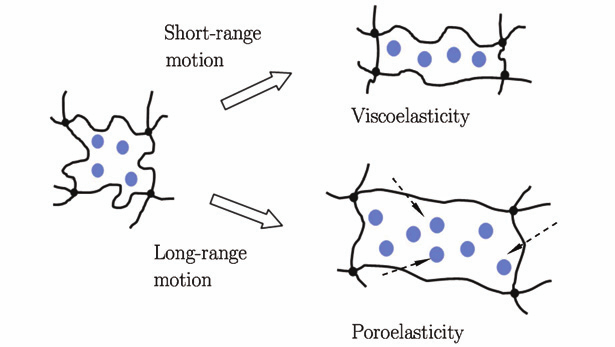
\includegraphics[scale=0.325]{images/visco_poro}
	\caption{Illustration of the molecular processes which account for the macroscopic deformation of ECM: viscosity is related to change in the conformation of the network which results in short-range movement of fluid relative to the polymers; poro-elasticity is instead responsible for the long-range diffusion of solvent molecules in the gel/tissue. Reproduced from \cite{viscoporo}.}
	\label{deformation}
\end{figure}
 
As mentioned in the introduction, we are here interested in the coupling of this two phenomena. As discussed in \cite{viscoporo}, there are spatial and time scales which allow to study the two independently. On one hand, nanoscale rheological testing with AFM give us information on the visco-elastic properties of the sample. For sufficiently small beads, the length scale considered in the experiment is so short that poroelastic relaxation is almost instantaneous and thus negligible. Different 1D rheological model are usually applied to fit experimental measurement: the most common for tissue and hydrogels is the \textit{Standard Linear Solid} model, which is illustrated in Figure \ref{figmode}(a), to fit the experimental data \cite{Article1,viscoporo}. The poro-elastic behaviour can instead be characterized by standard creep-relaxation test on whole sample. In this case, Darcy's law is usually applied to estimate the hydraulic conductivity and thus characterise the transport of fluid in the material \cite{Netti,viscoporo}. 

Despite having a good understanding of the two phenomena independently, there has been little attention to investigating how the two couple. In Figure \ref{figmode}, we have illustrated the two main approaches that have been proposed in the literature. To avoid any confusion, we will denote them as model A and model B respectively. Despite being quite similar, model B explicitly decouple the volumetric and deviatoric deformation of the system by introducing an addition spring to standard linear solid (SLS) \cite{magneto,NGUYEN,Jeru}. On the other hand, model A assumes that the model behaves as a SLS both under deviatoric and volumetric deformation.

At our knowledge, there is no systematic study in the literature that compares the two approaches and their predictions in different experiments. Instead of making an arbitrary decision, we will derive two models, one for each constitutive relation. We will then compare their predictions and investigate whether the two are consistent or can give rise to substantially different behaviour.    

As an explanatory example of the derivation of a model in the non-equilibrium thermodynamics framework, we will here fully derive the governing equation corresponding to model A. The interested reader can find the details of the derivation for model B in Appendix [Need to add the name]. 

\begin{figure}[h!]
	\centering
	\begin{subfigure}{0.32\textwidth}
		\centering
		\Large
	\def\svgwidth{0.95\linewidth}
	\input{latex/images/modelA1.pdf_tex}
	\caption{Rheological Model A}
	\label{fig1A}
	\end{subfigure}
	\begin{subfigure}{0.32\textwidth}
	\Large
	\def\svgwidth{0.95\linewidth}
	\input{latex/images/modelB1.pdf_tex}
	\caption{Rheological Model B}
	\label{fig1B}
\end{subfigure}

\begin{subfigure}{0.34\textwidth}
	\Large
	\def\svgwidth{1.75\linewidth}
	\input{latex/images/modelA2.pdf_tex}
	\caption{Multiplicative decomposition of Model A}
	\label{Model2}
\end{subfigure}
\vspace{5mm}
\caption{(a-b)two different rheological models for soft tissue; (c) multiplicative decomposition corresponding to model A, Equation~(\ref{dec1}).}
\label{figmode}
\end{figure}

Following a common approach in the large-deformation theory \cite{Article1,CACCAVO2,Plasto,magneto,NGUYEN,growthtum}, we base our derivation on a multiplicative decomposition of the deformation tensor $\F$, approach first proposed by Kr\"{o}ner in 1960 \cite{kro}:

\begin{equation}
\F=\F_e\F_v,\label{dec1}.
\end{equation}

As shown in Figure \ref{figmode}(a), $\F_e$ is the elastic contribution to the deformation related to the spring in branch $\mathbf{B}$. On the other hand, the term $\F_v$ accounts for the viscous flow due to the dashpot in branch $\mathbf{B}$. As illustrate in Figure \ref{figmode}(c), this multiplicative decomposition is equivalent to introducing an intermediate configuration $\mathcal{B}_v$, called natural or virtual configuration. Despite it not being a real state of the system, it can be interpreted as the state the system would be in if it was instantaneously elastically unload. 

Using Equation~(\ref{dec1}), we can compute the velocity gradient tensor $\LL$:
\begin{equation}
\LL = \dot{\F}\F^{-1} = \LL_e + \F_e \LL_v \F_e^{-1},
\end{equation}
where $\LL_e=\dot{\F}_e\F_e^{-1}$ and $\dot{\F}_v\F_v^{-1}$ are respectively the elastic and viscous velocity gradient tensor. These can be decomposed in their symmetric and skewed part:

\begin{equation}
\begin{aligned}
\LL_e = \mathbb{D}_e + \mathbb{W}_e, \ \ \mathbb{D}_e = \frac{\LL_e+\LL^T_e}{2}, \ \ \mathbb{W}_e = \frac{\LL_e-\LL^T_e}{2};\\
\LL_v = \mathbb{D}_v + \mathbb{W}_v,  \ \ \mathbb{D}_v = \frac{\LL_v+\LL^T_v}{2}, \ \ \mathbb{W}_v = \frac{\LL_v-\LL^T_v}{2}.
\end{aligned}
\end{equation}

The decomposition~(\ref{dec1}) is not unique, as stress state in $\mathcal{B}_v$ would not change under any arbitrary rigid-body rotation \cite{multdec}. As suggested by \cite{Plasto}, in the case of isotropic material, it is reasonable to assume the viscous flow to be irrotational, i.e. $\mathbb{W}_v=\mathbb{O}$, so that $\LL_v \equiv \mathbb{D}_v$.
As mentioned before, the physical nature of the viscous deformation, molecular rearrangement. This requires to introduce an additional constraint:
\begin{equation}
J_v=\det \F_v= 1.\label{Jv}
\end{equation}

Note that in the second model B, this condition is naturally imposed as the only volumetric contribution to the stress is related to $\F_{vol}$.
Despite condition~(\ref{Jv}) being common assumption in the study of hydrogels and soft tissue, there are few exceptions \cite{Article1,CACCAVO2,wang} model. Consequently, our results will differ from the one in the paper mentioned. 
 
\subsection{Energy Balance Inequality.}
As mentioned in Section \ref{secNET}, the energy imbalance inequality impose restrictions on the nature of the free energy $\psi$ depending on  how the system exchanges energy and mass with the environment. Considering a control volume $R$ in the reference configuration $\mathcal{B}_0$, the system exchanges mass due to diffusion of each mobile species, so that $M(R)$ is given by:
\begin{equation}
M(R)= \sum\limits_{m=s,1,\ldots,N} - \int_{\partial R} \mu_m \,\mathbf{J}_m \cdot \mathbf{n} 
\end{equation}
where $\mathbf{n}$ is the unit normal vector to the surface $\partial R$ and $\mu_m$ is the chemical potential associated with each species. Widely used in the thermodynamics of mixture, the chemical potential is a measure of the rate of change in free energy associated with adding one more molecule to a unit volume. The term $W(R)$, as defined in Section \ref{secNET}, is instead decomposed in two contributions, the rate of electrical $W_{el}(R)$ and mechanical work $W_{mec}(R)$. Following \cite{DROZDOVph}, $W_{el}(R)$ is defined as:
\begin{equation}
W_{el}(R) = -\int_{\partial R} \Phi\, \dot{\mathbf{H}}\cdot \mathbf{n}
\end{equation}
As suggested by Gurtin \cite{GURTIN}, when accounting for the mechanical work, besides the contribution of macro-stresses $\mathbb{S}$, we need also to account for the effect of micro-stresses $\boldsymbol{\epsilon}$, which arise due to the system heterogeneity \cite{microstress}. As before we only take into account the dominant contribution of the solvent while neglecting the solute, so that $W_{mec}(R)$ reads:
\begin{equation}
W_{mec}(R) = \int_{\partial R} \left(\boldsymbol{\xi}\cdot \mathbf{n}\right)\dot{C}_s + \int_{\partial R} \mathbb{S}\mathbf{n} \cdot \dot{\mathbf{u}}
\end{equation}
where $\mathbf{u}= \mathbf{x}-\mathbf{X}$ is the displacement vector, which is related to the deformation tensor by $\F=\mathbb{I}-\nabla_0 \mathbf{u}$. Substituting this result back into the formula~(\ref{energyin}) and applying the divergence theorem we obtain the following integral inequality:
\begin{equation}
\int_R \dot{\psi} - \mathbf{E}\cdot \dot{\mathbf{H}} \, + \, \sum\limits_{i=1}^{N} \left[e \Phi  z_i \dot{C}_i+ \nabla_0 \left(\mu_i \mathbf{J}_i \right)\right] + \nabla_0 (\mu_s \mathbf{J}_s- \boldsymbol{\xi}\dot{C}_s -\mathbb{S}^T\mathbf{\dot{u}}) \leq 0 
\end{equation}
Since the above inequality must hold for any choice of the volume $R$, the constraint must hold locally. So that:
\begin{equation}
\dot{\psi} - \mathbf{E}\cdot \dot{\mathbf{H}} \, + \, \sum\limits_{i=1}^{N} \left[e \Phi  z_i \dot{C}_i+ \nabla_0 \left(\mu_i \mathbf{J}_i \right)\right] + \nabla_0 (\mu_s \mathbf{J}_s- \boldsymbol{\xi}\dot{C}_s -\mathbb{S}^T\mathbf{\dot{u}}) \leq 0. 
\end{equation}
Further accounting for Equations~(\ref{consmass})-(\ref{consmom}), we obtain that:
\begin{equation}
\begin{aligned}
\dot{\psi} - \mathbf{E}\cdot \dot{\mathbf{H}} \, + \, \sum\limits_{i=1}^{N} \left[e \Phi  z_i - \mu_i\right] \dot{C}_i - (\mu_s + \nabla_0 \cdot \boldsymbol{\xi})\,\dot{C}_s -\mathbb{S}:\dot{\F}\\
-\boldsymbol{\xi} \cdot \nabla_0 \, \dot{C}_s + \sum\limits_{m} \nabla_0 \, \mu_m \cdot \mathbf{J}_m \leq 0.
\label{temp2}
\end{aligned} 
\end{equation}

As exhaustively discussed in previous studies \cite{Plasto,GURTIN}, the energy imbalance inequality impose restrictions on the constitutive equation of the free energy $\psi$. Adapting their results, to our specific problem, we have that:
\begin{equation}
\psi = \psi (\F,\F_e, C_s, C_i, \nabla_0 \,C_s,\mathbf{H}), \label{temp1}
\end{equation}
which rules out preclude any explicit dependency of $\psi$ on the chemical potential or the viscous deformation gradient $\F_v$. By differentiating the incompressibility condition~(\ref{inc}), we obtain:
\begin{gather}
v_s\dot{C_s} - J \F^{-T}:\dot{\F} =0 \label{temp3}.
\end{gather}

The condition~(\ref{Jv}) will be instead strongly imposed. [REPHRASE]
If we now substitute~(\ref{temp1}) into~(\ref{temp2}), and include the constraint~(\ref{temp3}) using $p$ as Lagrange multiplier, we are left with the augmented form of the energy imbalance inequality:
\begin{equation}
\begin{aligned}
\left(\frac{\partial \psi}{\partial \nabla_0 C_s}-\boldsymbol{\xi}\right) \cdot \nabla_0 \dot{C}_s + \left(\frac{\partial \psi}{\partial C_s}-\mu_s-\nabla_0 \cdot \boldsymbol{\xi}+p v\right)\dot{C}_s\\
+ \sum_i\left(\frac{\partial \psi}{\partial C_i} + e\Phi z_i-\mu_i\right) \dot{C}_i +\left(\frac{\partial \psi}{\partial \mathbf{H}}-\mathbf{E}\right) \cdot \dot{\mathbf{H}}\\
+ \left(\frac{\partial \psi}{\partial \F} + \frac{\partial \psi}{\partial\F_e}\F_v^{-1}- \mathbb{S} - p J \F^{-T}\right): \dot{\F}+ \sum_m \nabla_0 \,\mu_m \cdot \mathbf{J}_m \\
- \left(\F_e^T\frac{\partial \psi}{\partial \F_e}+p_v\mathbb{I}\right):\mathbb{L}_v\leq 0 . \label{ineq}
\end{aligned}
\end{equation}

Note that in deriving~(\ref{ineq}), we have also made us of the following identity:
\begin{equation}
\dot{\F}=\dot{\F}_e\F_v+\F_e\dot{\F}_v \Longrightarrow \dot{\F}_e=\dot{\F}\F_v^{-1}-\F_e \LL_v.
\end{equation}

\subsection{Entropy Production $\sigma$.}

Having specified how the system interact with its environment, we can now discuss how it dissipates energy. As mentioned in Section~(\ref{}), there are two contributions: transport (diffusion of solvent and solutes) and viscosity. The thermodynamic fluxes \footnote{See Section \ref{secNET}} associated with these two phenomena are $\mathbf{J}_m$, $m=s,1,\ldots,N$, and $\LL_v$. Consequently, using Equation~(\ref{2law}), we obtain:
\begin{equation}
\sigma = \sum_m \zeta_m \cdot \mathbf{J}_m + \zeta_v : \LL_v,
\label{dis}
\end{equation}
where $\zeta$s represent the thermodynamic forces associate with each flux. 

Based on Equations~(\ref{eqCIT}), (\ref{ineq}) and (\ref{dis}), we can move from the energy imbalance to an equality condition:
\begin{equation}
\begin{aligned}
\left(\frac{\partial \psi}{\partial \nabla_0 C_s}-\boldsymbol{\xi}\right) \cdot \nabla_0 \dot{C}_s + \left(\frac{\partial \psi}{\partial C_s}-\mu_s-\nabla_0 \cdot \boldsymbol{\xi}+p v\right)\dot{C}_s\\
+ \sum_i\left(\frac{\partial \psi}{\partial C_i} + e\Phi z_i-\mu_i\right) \dot{C}_i +\left(\frac{\partial \psi}{\partial \mathbf{H}}-\mathbf{E}\right) \cdot \dot{\mathbf{H}}\\
+ \left(\frac{\partial \psi}{\partial \F} + \frac{\partial \psi}{\partial\F_e}\F_v^{-1}- \mathbb{S} - p J \F^{-T}\right): \dot{\F}+ \sum_m \left[\nabla_0 \,\mu_m - \zeta_m\right]\cdot \mathbf{J}_m \\
-\left[\zeta_v + \left(\F_e^T\frac{\partial \psi}{\partial \F_e}-p_v\mathbb{I}\right)\right]:\mathbb{L}_v=0
\end{aligned} 
\end{equation}
which needs to hold for any possible value of the fluxes of the thermodynamics variables
\subsection{Construction of the Free Energy.}

Following a standard approach in phase-field modeling, we assume that the total free energy can be additively decomposed, so that each mechanisms contributes independently:

\begin{enumerate}
	{\indentitem\item[\textbullet] the energy of the electric field $\psi_1$;}
	{\indentitem \item[\textbullet] the energy of solvent and solutes' molecules not interacting with the solid phase $\psi_2$;}
	{\indentitem\item[\textbullet] the energy of mixing the solid phase with the solution, $\psi_3$;}
	{\indentitem\item[\textbullet] the energy of mixing the solvent with the solutes in solution, $\psi_4$;}
	{\indentitem\item[\textbullet] the interfacial energy between dissimilar phases, $\psi_5$;}
	{\indentitem\item[\textbullet] the energy of the solid phase not interacting with the solution, $\psi_6$.}
\end{enumerate}

Assuming the solid phase to be an ideal and linear dielectric material, with constant permittivity $\epsilon$,the free energy of polarization reads \cite{DROZDOV+,Reviewpolyel}:
\begin{gather}
\psi_1 = \frac{1}{2\epsilon J} \mathbf{H}\F^T \cdot \F \mathbf{H}.
\end{gather}

The specific energy density $\psi_2$ has the standard form:
\begin{equation}
\psi_1 = \sum\limits_{m} \mu^0_m C_m
\end{equation} 
where $\mu^0_m$ denotes the chemical potential of non interacting solvent and ions molecules. According to Flory-Huggins theory \cite{flory,hug} of mixtures, the mixing energy is given by:
\begin{equation}
\psi_3 = \frac{k_B T J}{v_s} \left(\phi_f \ln \phi_f + \chi \phi_f \phi_n\right),
\end{equation}
where $k_B$ is the Boltzmann's constant, $T$ is the temperature and $\chi$ is the Flory-Huggins parameter, which is related to the enthalpy of mixing. It is worth mentioning that Xue et al. follow a different approach \cite{ecm1,ecm2}. They assume that only the mixing of GAGs and solvent contributes to the free energy. Despite the swelling properties of the ECM are mainly related to GAGs, we could find no direct experimental evidence that collagen can not mixing with water. Moreover, as mentioned in Section \ref{ECMcomp}, we are not considering GAGs and collagen as separate entities, but as a unique solid phase.

As the interstitial fluid is well approximated by a dilute solution, the contribution $\psi_4$ reads \cite{Reviewpolyel,ecm1,ecm2}:

\begin{equation}
\psi_4 = k_B T \sum\limits_{i=1}^{N} C_i \left(\ln \frac{C_i}{ C_s}-1\right).
\end{equation}

As proposed by Hong et al. \cite{Interface}, we include in the energy the effect of interface tension. Despite having been neglected in many models for hydrogel swelling, this term plays a role in the transient poroelastic relaxation of the material, when boundaries between solvent-rich and solvent-poor regions can emerge \cite{sarah,Interface}. Again we assume that the contribution of mobile ions is negligible, so that only the ideal solid-solvent interface contributes to the energy:
\begin{equation}
\psi_5 = \frac{\gamma}{2} J \left|\nabla C_s\right|,
\end{equation}
where the constant $\gamma$ plays a role analogous to a surface tension. Without any loss of generality we assume that the last term $\psi_6$ in the free energy can be additively decomposed into two contribution; one for each branch of the standard linear solid model in Figure \ref{figmode} (a):

\begin{equation}
\psi_6 = \psi_\mathbf{A}(\F) + \psi_\mathbf{B}(\F_e).
\end{equation}

As in \cite{ecm2}, we decide to model the solid network as an isotropic and compressible Neo-Hookean material:

\begin{eqnarray}
\psi_\mathbf{A}(\F) = \frac{G_\mathbf{A}}{2} \left(\F:\F - 3 -2 \ln J\right)\\
\psi_\mathbf{B}(\F_e) = \frac{G_\mathbf{B}}{2} \left(\F_e:\F_e - 3 -2 \ln J_{e}\right)\label{hyp}
\end{eqnarray}
where $G_\mathbf{\cdot}$ stands for the shear modulus associated with each branches, $J_e= \det \F_e$, while $J$ is as defined in the previous sections. As derived in \cite{floryprinciples}, the hyper-elastic model~(\ref{hyp}) can be correlated to the microscopic properties of a polymer network, under the assumption of Gaussian chains and affine deformation. Other thermodynamically consistent form of the stretching energy have been proposed in the literature \cite{BERGSTROM1998931,boyce2,doi}. These have been also derived by statistical arguments but starting from different network models.

\newpage
\bibliographystyle{splncs04}
\bibliography{latex/ref}
%
\end{document}
